\documentclass[12pt]{article}
\usepackage{amsfonts}
\usepackage{graphicx}

%%%%%%%%%%%%%%%%%%%%%%%%%%%%%%%%%%%%%%%%%%%%%%%%%%%%%%%%%%%%%%%%
%
% dimensions choisies par l'utilisateur (bricolage personnel)

\newdimen\decalage

\paperheight=29.7 true cm \paperwidth=21 true cm
\textheight=25.7 true cm \textwidth=17 true cm
\decalage=0 true cm

% déduction de \topmargin,
% \evensidemargin et \oddsidemargin

\oddsidemargin=\paperwidth
\advance\oddsidemargin by -\textwidth
\divide\oddsidemargin by 2
\advance\oddsidemargin by -1 in
\evensidemargin=\oddsidemargin
\advance\oddsidemargin by \decalage 
\advance\evensidemargin by -\decalage

\topmargin=\paperheight
\advance\topmargin by -\headheight
\advance\topmargin by -\headsep
\advance\topmargin by -\textheight
\advance\topmargin by -\footskip
\divide\topmargin by 2
\advance\topmargin by -1 in

%
%%%%%%%%%%%%%%%%%%%%%%%%%%%%%%%%%%%%%%%%%%%%%%%%%%%%%%%%%%%%%%%%

\begin{document}

\title{Compte rendu du TP4 - Fourier}
\author{Louis Allain}
\maketitle

\section{Transformée de Fourier 2}

\subsection{Transformée de Fourier appliquée à des signaux sonores réels}

Réponses aux question :
\begin{enumerate}
	\item 
		En ayant pris le son fourni de la corneille noire "`corneillenoire.wav"', voici les résultats :
		\begin{verbatim}
			taille du fichier :  26067
			fréquence d'échantillonnage :  8000
			durée du signal :  3.258375 s
		\end{verbatim}
		
	\item
		Voici un affichage en amplitude du spectre complet du signal : 
		$$
			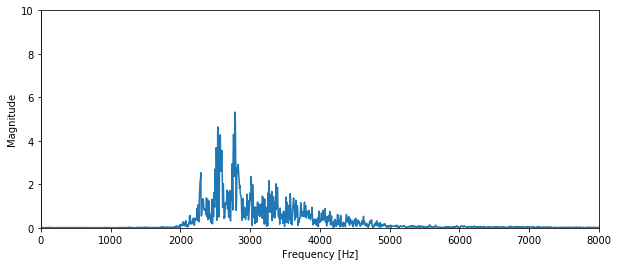
\includegraphics[width=0.8\textwidth]{q2_amplitude.png}
		$$
		Voici un autre affichage en amplitude du spectre du signal avec un offset égal à 2500 et une fenêtre de 512 :
		$$
			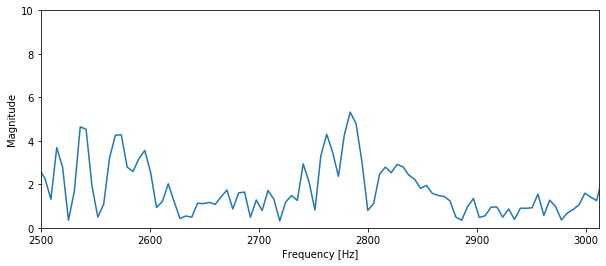
\includegraphics[width=0.8\textwidth]{q2_amplitude_1.png}
		$$
		Voici un affichage de la phase du spectre avec un offset 100 et une fenêtre de 512 :
		$$
			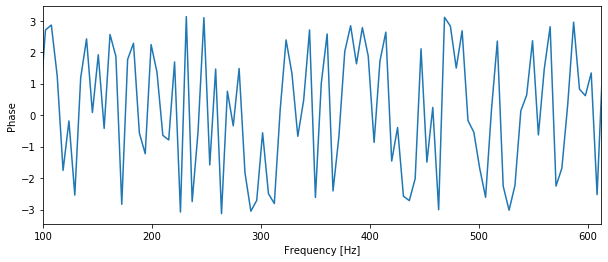
\includegraphics[width=0.8\textwidth]{q2_phase_1.png}
		$$
		Voici un affichage de la phase du spectre avec un offset 100 et une fenêtre de 128 :
		$$
			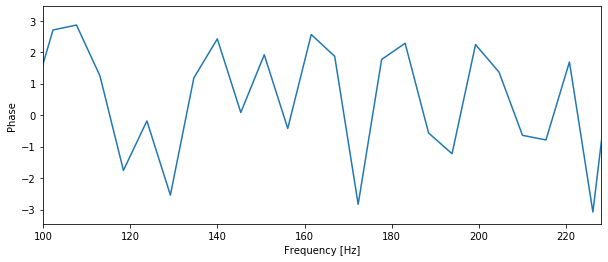
\includegraphics[width=0.8\textwidth]{q2_phase_2.png}
		$$
		
	\item
		Traçage du spectrogramme du signal :
		$$
			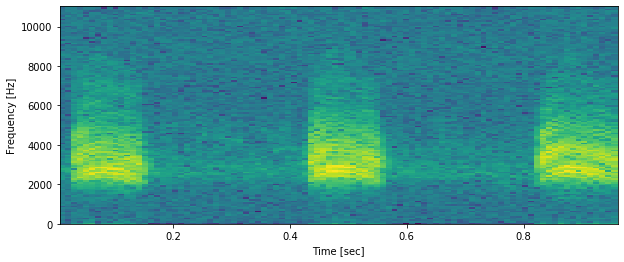
\includegraphics[width=0.8\textwidth]{q3_spectrogramme.png}
		$$
		
	\item
		Voici la fonction calculerSpectre qui renvoie le vecteur fréquentiel et lecteur du spectre (en dB ou non) :
		\begin{verbatim}
			def calculerSpectre(echantillons, fs, dB=False):
    
					N = echantillons.size
					sf = np.zeros(N)
					sf[:] = echantillons[0:N]
					X = fft(sf)/N # tfd
					F = np.linspace(0, fs, N)
					
					if(dB): 
							X = 10 * np.log10(abs(X)) # dB
					
					return (F, X)
		\end{verbatim}
		De plus voici, par exemple le résultat de la fonction. On affiche ici le spectre en dB en fonction de la fréquence :
		$$
			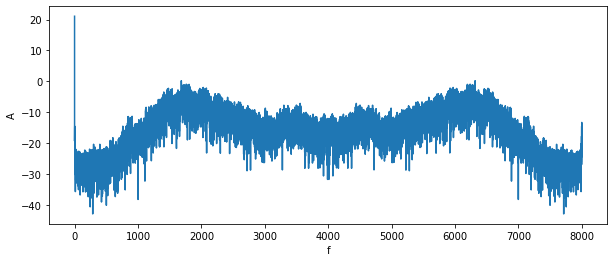
\includegraphics[width=0.8\textwidth]{q4_calculerSpectre_dB.png}
		$$
		
	\item
	
		Voici la fonction movingFFT :
		\begin{verbatim}
			def movingFFT(filename, winsize, offset, wintype):
					(fs, x) = read(filename)
					(freq, spectre) = calculerSpectre(x, fs, False)
					N = x.size
					plt.figure(figsize=(10,4))
					plt.xlim(offset, winsize+offset)
					plt.ylim(-0.5, 0.5)
					spectre = spectre*signal.get_window(wintype,N)
					plt.plot(freq, spectre)
				
		\end{verbatim}
		Et voici le résultat de cette fonction sur le fichier piebavarde.wav avec un offet de 2600 et une fenêtre de 256 :
		$$
			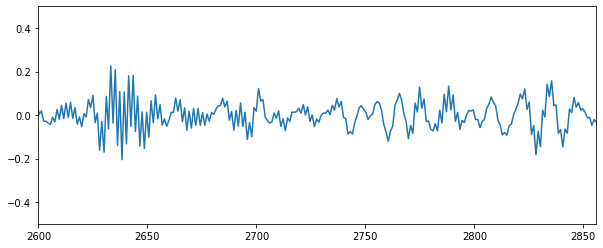
\includegraphics[width=0.8\textwidth]{q5_movingFFT.png}
		$$
		
\end{enumerate}
\end{document}